\documentclass[9pt]{article}
\textwidth 6.65truein
\textheight 9.5truein
\oddsidemargin -0.2in
\topmargin -0.6in
\usepackage{amssymb,amsmath}
\usepackage{amsthm}
\usepackage{graphicx}
\usepackage{hyperref}
\usepackage{natbib}
\usepackage[lined,boxed,commentsnumbered]{algorithm2e}
%\usepackage[lined,commentsnumbered]{algorithm2e}

%-------------------------------------------------
\begin{document}
\newtheorem{theorem}{Theorem}
\newtheorem{lemma}{Lemma}
\newtheorem{remark}{Remark}
\newtheorem{definition}{Definition}
%\newenvironment{proof} {\noindent{\bf Proof:}} {$\square$\\}
\newenvironment{ml}[1] {
   \noindent {\bf #1}:
   %\indent
   \begin{enumerate}
}{
   %$\square$ \\
   \end{enumerate}
}
\newenvironment{mlr}[1] {
   {{\it ---(#1)}:}} {
}
%--------------------------------------------------

\title{Drop connect layer in neural network}
\author{LI WAN}
\date{\today}
\maketitle
%----------------------------------------------
\section{Motivation}
In neural network, fully connected layer, 
Given input $x=[x_1,x_2,\ldots,x_{n-1}, 1]^T$, and layer parameters
$W$(of size $m\times n$), the output $y=[y_1,y_2,\ldots,y_m]^T$
of is computed as follows with activation function $f$:
\begin{equation}
   \label{eqn:fcfprop}
   y = f(Wx) = f(\sum_i x_i W_{.i})
\end{equation}

\subsection{Dropout}
Drop Out was proposed by ~\cite{hinton2012} which says the output of some
layer of network have $1-p$ chance to set to $0$ and $p$ chance remain unchanged ($1-p$
is call drop rate).
They claim that such idea is good to improved network's generalization
ability and they empirical result validate their claim.

Applying such idea to such fully connected neuron,
we have each $y_j$ with some probability of either being $y_j$ or $0$.
Combine this with Equation~\ref{eqn:fcfprop}:
\begin{equation}
   \label{eqn:fcdrop}
   y=\delta*f(Wx) 
\end{equation}
, where  $*$ denotes element wise produce and $\delta$ 
   is a vector of size $n$ with  $\delta_j\sim Bern(p)$

It is known that most of commonly used activation function $f$ is a 
function with $f(0)=0$, for example $tanh$,$sigmod$ and $relu$ all have such property. 
Equation~\ref{eqn:fcdrop} could be re-written as:
\begin{equation}
   \label{eqn:fcdropo}
   y=f(\delta *Wx) = 
   f\left( \sum_{i=1}^n x_i \left(\delta*W_{.i}\right)\right)
   =
   f\left( \sum_{i=1}^n x_i 
   \begin{bmatrix}
   w_{1i}\delta_1 \\
   w_{2i}\delta_2 \\ 
   \ldots, \\
   w_{ni}\delta_n
   \end{bmatrix}
    \right)
   \mbox{ where  } \delta_j\sim Bern(p)
\end{equation}

\subsection{Drop connect}
Similar with Drop output, drop connect says each connection is dropped with
probability $p$. Drop output bring us a sparse activation function and drop
connection bring us a sparse connected matrix. In other words, fully connected layer
with drop connect will become sparse connected matrix but the connection is
{\it random} for each fprop training. 
This is not the same as set $W$ to sparse matrix, 
in that case, $W$ is {\it fixed} for each fprop training. 

We believe that such
randomness have the similar property with drop output idea: better 
generalization ability and empirical study of drop connect layer will be given
in experiment section.
In drop connect layer, the fprop formula is given as:
\begin{equation}
   \label{eqn:fcdropc}
   y = f\begin{bmatrix}
      (W_{1.}*\delta_{1.})x \\
      (W_{2.}*\delta_{2.})x \\
      \ldots \\
      (W_{m.}*\delta_{m.})x 
   \end{bmatrix}
   = f\left(\left(W*\delta\right)x\right) = 
   f\left(
   \sum_{i=1}^n x_i 
   \begin{bmatrix}
      w_{1i}\delta_{1i} \\ 
      w_{2i}\delta_{2i} \\ 
      \ldots \\ 
      w_{ni}\delta_{ni}
    \end{bmatrix}
    \right)
\end{equation}
, where $\delta$ is a binary matrix the same size as $W$ and 
$\delta_{ji}\sim Bern(p)$

Compare Equation~\ref{eqn:fcdropc} and ~\ref{eqn:fcdropo}, we could easily see that
the drop-connect is a generalization of drop-output by set $\delta_{ji}$ in 
Equation~\ref{eqn:fcdropc} to $\delta_i$ in Equation~\ref{eqn:fcdropo}.

%\subsection{Approximate Inference drop connect by Normal Distribution}
%drop connect requires us to generate a random matrix $\delta$ for each instance $x$. This is not easy to parallelize
%because each input $x$ will be multiple a different weight matrix $\delta*W$. We could approximate the output of drop
%connection by Gaussian distribution via moment matching. 
Let $z$ denotes the output of layer before applying 
neuron transformation, thus $y=f(z)$. According to Equation~\ref{eqn:fcdropc}, we have
$$
E[z] = E[ (W*\delta)x ] = 
   \sum_{i=1}^n x_i 
   \begin{bmatrix}
      w_{1i}E[\delta_{1i}] \\ 
      w_{2i}E[\delta_{2i}] \\ 
      \ldots \\ 
      w_{ni}E[\delta_{ni}]
    \end{bmatrix} = pWx
$$
and
$$
Var[z]= Var[ (W*\delta)x ] = 
   \sum_{i=1}^n x_i^2
   \begin{bmatrix}
      w_{1i}^2Var[\delta_{1i}] \\ 
      w_{2i}^2Var[\delta_{2i}] \\ 
      \ldots \\ 
      w_{ni}^2Var[\delta_{ni}]
    \end{bmatrix} = p(1-p) (W*W)(x*x)
$$
Thus output before neuron activation $z$ follows a normal distribution described as:
\begin{equation}
   \label{eqn:dropc_normal}
   z\sim {\mathit N}\left( pWx, p(1-p)(W*W)(x*x) \right)
\end{equation}
%----------------------------------------------
\section{Model Description}
\label{sec:description}
This section will formally describe drop-connect model: using drop connect 
layer as an replacement for fully connect layer in neural network. 
\begin{definition}[Weighted Mixture Model]
   \label{def:mixture_model}
   Given data set $S$ with $\ell$ entries: 
   $\{{\bf x}_1,{\bf x}_2,\ldots,{\bf x}_{\ell}\}$ with label 
   $\{y_1,y_2,\ldots,y_{\ell}\}$, we define the following mixture of classifier model:
   \begin{equation}
      \label{eqn:model}
      {\bf u} = \sum_{m}p(m) f({\bf x};w,m)=\mathbf{E}_{m}\left[f({\bf x};w,m)\right]
   \end{equation}
   where each classifier $f(x;w,m)$ has weights $p(m)$.
\end{definition}

\begin{remark}
    when each element of $m_i$ has equal probability of being on and off ($p=0.5$), the mixture model
    has equal weights for all sub-models $f(\mathbf{x};w,m)$, otherwise the mixture model
    has larger weights in some sub-model than others.
\end{remark}

\begin{definition}[drop-connect Neural Network]
   \label{def:dropc_nn}
   drop-connect Neural Network (Figure~\ref{fig:model})
   is a special case of Weighted Mixture Mode (Definition~\ref{def:mixture_model})
   where $f$ is a neural network and random vector $m$ defines the connection activation statues
   in drop-connect layer. The network includes the following parts:
   \begin{enumerate}
      \item Feature Extractor: ${\mathbf v}=g({\mathbf x})$ where $v$ are the 
         features and $\mathbf x$ is input. 
      \item drop connect Layer: $\mathbf{z} = a(h({\mathbf v};w,m))$ 
         where $a$ is non-linear activation
         function and $h$ computes network response given 
         input $\mathbf v$ and weights $\mathbf w$.
         Each element of $m$ defined the activation status of corresponding weights:
         $$
         m_i=
         \left\{
            \begin{array}{ll}
               1 & \mbox{ with prob $p$ ($w_i$ is active)}\\
               0 & \mbox{ with prob $1-p$ ($w_i$ is not active)}
            \end{array}
            \right.
         $$
     \item Dimension Reduction: $\mathbf{u}=s(\mathbf{z})$. Reduce feature dimension from 
         drop-connect layer to number of labels
   \end{enumerate}
   Thus, drop-connect neural network prediction function is as follows (
   from Equation~\ref{eqn:model}):
   \begin{equation}
      \label{eqn:nnmodel}
      \mathbf{u} = \mathbf{E}\left[ f(\mathbf{x};w,m\right]
      = \mathbf{E}\left[ s\circ a\circ h_{m}\circ g(\mathbf{x};w)\right]
   \end{equation}

\end{definition}
\begin{figure}[ht]
   \label{fig:model}
   \centering{
      \includegraphics[width=3.2in]{figs/model2.eps}
   }
   \caption{
      Drop connect Neural Network Model $u=f(x)$, where 
      $f=s\circ a\circ h\circ g$:
      a) feature extractor: $v=g(x)$ 
      b) drop connect layer:
      $z=a(h(v;w,m))$ with activation function $a$ and drop connect
      layer function $h$ parametrized by a fixed vector$w$ and a random vector $m$
      c) dimension reduction: $u=s(z)$
   }
\end{figure}
\begin{remark}
   Definition~\ref{def:dropc_nn} defines network with only one drop-connect
   layer for simplicity. Extends to multiple drop-connect layers are straight forward.
\end{remark}
\begin{remark}
   Nonlinear property in network is very important. Consider another special case of
   Weighted Mixture Model (Definition~\ref{def:mixture_model}): mixture of
   linear classifier (binary prediction) defined as follows:
   \begin{equation}
      \label{eqn:logistic_classifier}
      \mathbf{u}= \mathbf{E}_m\left[f({\mathbf x};w,m)\right] = 
      \mathbf{E}_m\left[\sum_{i=1}^n x_{i}w_{i}m_i+bm_b\right]=
      \sum_{i=1}^nx_iw_i\mathbf{E}\left[m_i\right]
      + b\mathbf{E}\left[m_i\right]
      =p(w^Tx+b)
   \end{equation}
\end{remark}

\begin{definition}[Logistic Loss Function]
The following loss function is call logistic loss function:
\begin{equation}
   \label{eqn:loss}
   A(u)=A(x-y)=-\sum_i y_i \ln \frac{\exp(x_i)}{\sum_j \exp(x_j)}=y^Tx-\ln\sum_j\exp(x_j)
\end{equation}
where 
%$y$ is a binary vector with $u_i<0$ bit on and $x$ is a real vector with:
$$
x_i=\left\{
    \begin{array}{ll}
        1+u_i & \mbox{ if $u_i<0$ } \\
         u_i & \mbox{ otherwise}
    \end{array}
    \right.
\mbox{  and    }
y_i = \left\{
    \begin{array}{ll}
        1 & \mbox{ if $u_i<0$ } \\
        0 & \mbox{ otherwise}
    \end{array}
    \right.
$$
\end{definition}

\begin{remark}[Softmax layer]
    Softmax layer in neural network with input $x$ output $u_i$ and parameter $w_i$ ($i=1,2,\ldots,n$):
    $$
    u_i = \frac{\exp{(w_i^Tx)}}{\sum_j \exp{(w_j^Tx)}}
    $$
    and cross entropy loss function is identical with combine Dimension Reduction in Definition~\ref{def:dropc_nn} 
    and logistic loss function.
\end{remark}

\begin{definition}[Empirical Loss]
The overall loss function of training set $S$ is, this is also called empirical loss:
\begin{equation}
   \label{eqn:loss2}
   L(w) = \frac{1}{2}\lambda \|w\|^2_2 + \sum_{i=1}^\ell A( u_i-y_i )
\end{equation}
where $y$ is binary vector representation of label information and $u$ is output of network.
\end{definition}

We present an algorithm listed in Algorithm~\ref{alg:train} to minimize empirical loss
of drop connect network. There is no much different between Algorithm~\ref{alg:train}  
and standard sgd algorithm except we are 
going to random sample $m$ every time for each $x_i$. However, the loss function defined
in Equation~\ref{eqn:loss2} and Equation~\ref{eqn:nnmodel} involves sum of all possible
cases of $m$, the number of terms here is $2^{dim(m)}$. Further more, we could not
apply the trick shown Equation~\ref{eqn:logistic_classifier} for find a simple close form
because of non-linearity of $f$ (This is desired property). 

In Section~\ref{sec:convergence}, we are going to show
Algorithm~\ref{alg:train} indeed converges to a local minimal of empirical loss. 
The relationship between random sample parameter $p$ and generalization bound is given in
Section~\ref{sec:bound}.
\begin{algorithm}[ht]
   \label{alg:train}
   \caption{Stochastic Gradient Descent for Training Network with Drop-connect Layers}
   \KwIn{data set $S$}
   \KwOut{neural network weights $w$}
   $L_0\leftarrow \infty$\;
   \While{ $|L_{t}-L_{t-1}|<\epsilon $ }
   {
      $t\leftarrow t+1$\;
      $L_t\leftarrow 0$\;
      \For{$i\in 1,2,\ldots, \ell$} {
         random sample $m^i$: $m^i_j\sim Bern(p)$\;
         $L_t^i\leftarrow A( u_iy_i)$\;
         $w\leftarrow w - \eta \frac{\partial L_t^i}{\partial w}$\;
         $L_t\leftarrow L_t + L_t^i$\;
      }
   }
\end{algorithm}


%---------------------------------------
\section{Model Analysis}
\subsection{Convergence}
\label{sec:convergence}
\begin{theorem}
   \label{thm:converge}
   Algorithm~\ref{alg:train} actually minimize the empirical loss defined by
   by Equation~\ref{eqn:nnmodel} and Equation~\ref{eqn:loss2} for training data of neural network
\end{theorem}
\begin{proof}
   Substitute Equation~\ref{eqn:model} into Equation~\ref{eqn:loss2}:
\begin{eqnarray}
   L(w) &=& \lambda\|w\|_2 +\sum_{i=1}^\ell A(y_iu_i) 
   = \lambda\|w\|_2 +\sum_{i=1}^\ell A\left( y_i \mathbf{E}_m\left[f\left({\bf x};w,m\right)\right]\right) \nonumber \\
   &\leq &
   \lambda\|w\|_2 +\sum_{i=1}^\ell \mathbf{E}_m\left[A\left( f\left({\bf x}_i;w,m\right)-y_i \right)\right] \label{eqn:loss_bound_1} \\
   &=&
   \lambda\|w\|_2 +\mathbf{E}_{x,m}\left[A\left( f\left({\bf x};w,m\right)-y \right) \right]\label{eqn:loss_bound_2} \\
\end{eqnarray}
\begin{itemize}
   \item Equation~\ref{eqn:loss_bound_1} is because $A(x)$ is convex function ($A''(x)>0$)
   \item Equation~\ref{eqn:loss_bound_2} shows overall loss could be bounded by expected loss
       of $x,m$. Algorithm~\ref{alg:train} used individual sample gradient 
       to approximate overall expected gradient (the same as sgd).
   \end{itemize}
\end{proof}


\begin{theorem}
   \label{thm:converge_speed}
   Define the following operations on bit vector $m_1$ and $m_2$:
   \begin{enumerate}
       \item Set intersection operator $m=m_1\cap m_2$: $m(i)=1$ iff $m_1(i)=1$ and $m_2(i)=1$
       \item Set minus operator $m=m_1\setminus m_2$: $m(i)=1$ iff $m_1(i)=1$ and $m_2(i)\neq 1$
   \end{enumerate}
      Define function $I$ on bit vector $m$: $I(m)=\sum_j \delta(m_j,1)$.
   Algorithm~\ref{alg:train} updates $p^2$ dimension of mixture model on average in each step, i.e.
   $$
   {\mathbf E}_{m^i}\left[\sum_{m^j} p(m^j) \frac{I(m^j\cap m^i)}{I(m^j)}\right]=p^2
   $$
\end{theorem}
\begin{proof}
    For any $m\neq m^i$, we could decompose $m$ as 
    $m= \left(m\cap m^i\right) + \left(m\setminus m^i\right)$ and let $d_i=I(m_i)$ and $n=dim(m)$
   \begin{eqnarray}
      {\mathbf E}_{m^i}\left[\sum_{m} p(m) \frac{I(m\cap m^i)}{I(m)}\right]
      &=& {\mathbf E}_{m^j}\left[{\mathbf E}_{m^i}\left[\frac{I(m^j\cap m^i)}{I(m^j)}\right]\right]  \nonumber \\
      &=& {\mathbf E}_{m^j}\left[ \sum_{i=0}^{d_j}\binom{d_j}{i}{(1-p)^{d_j-i}p^i}\frac{i}{d_j}\right] \label{eqn:bit_update1} \\
      &=& {\mathbf E}_{m^j}\left[ pd_j\right]=p^2 \label{eqn:bit_update2}
   \end{eqnarray}
   \begin{itemize}
      \item Given a fixed bit vector $m_j$, there are $\binom{d_j}{i}$ set of vectors intersect with $m_j$ have $i$ bits on
         each of them have with probability $(1-p)^{d_j-i}p^i$ (Equation~\ref{eqn:bit_update1}).
      \item 
         $\sum_{i=0}^{d_j}\binom{d_j}{i}{(1-p)^{d_j-i}p^i}i$ is the expectation of number of bit on for a bit vector of size $d_j$,
         thus $\sum_{i=0}^{d_j}\binom{d_j}{i}{(1-p)^{d_j-i}p^i}i=pd_j$
         (Equation~\ref{eqn:bit_update2}).
   \end{itemize}
\end{proof}
\begin{remark}
   It is known that sgd algorithm converges to local minimal linearly, but 
   Theorem~\ref{thm:converge_speed} tells about convergence speed between
   network with/without drop connect layer for a fixed learning rate. If you
   find a good learning rate $\eta$ for a fully connected layer, the network $p^2$ times
   slower if you switch such fully connected layer to drop connect layer. 
\end{remark}

%-----------------------------------------------
\subsection{Inference}
\label{sec:inference}
In neural network, $s$ function is just an linear transformation, 
thus we could rewrite
Equation~\ref{eqn:nnmodel} as:
$$
\mathbf{E}_m[f(\mathbf{x};w,m)]=s(\mathbf{E}_m[a\circ h_m\circ g(x)])
$$
A simple way~\cite{hinton2012} to approximate above equation for fast inference is:
$$
s(\mathbf{E}_m[a\circ h_m\circ g(x)])\approx
s(a\circ \mathbf{E}_m[h_m\circ g(x)])
$$
such approximation is good only if $a$ is differentiable everywhere, because:
$$
\mathbf{E}[f(x)] = f(\mu_x) + f''(\epsilon)(x-\mu_x)^2 \mbox{ where  } \epsilon\in [x,\mu_x]
$$
However, such approximation is not good for ReLU neuron~\cite{Nair2010}. 
Let $x\sim \mathcal{N}(0,1)$ and $a(x)$ be ReLU neuron defined as follows:
$$
a(x)=\left\{
    \begin{array}{ll}
        x & \mbox{ when } x>0\\
        0 & \mbox{ otherwise}
    \end{array}
    \right.
$$
It is not hard to show that $E[a(x)]=1/\sqrt{2\pi}\approx 0.4$ in this case.

Algorithm~\ref{alg:inference} gives and Monte Carol sampling algorithm 
for inference network with drop-connect layers.
\begin{algorithm}[ht]
    \label{alg:inference}
    \caption{Inference Network with Drop-connect Layers }
    \KwIn{a new example $x$, neural network weights $w$}
    \KwOut{prediction $u$}
    $v\leftarrow g(x)$\;
    $\mu_r\leftarrow \mathbf{E}_m[h(v;w,m)]$\;
    $\sigma_r^2\leftarrow {\mathbf{Var}_m[h(v;w,m)]}$\;
    \While{ $i<\ell$ }{
        random sample $r_i\sim \mathcal{N}(\mu_r,\sigma_r^2)$\;
        $z_i\leftarrow a(r_i)$\;
    }
    $u=s(\sum_{i=1}^{\ell} z_i)$\;
\end{algorithm}
\begin{theorem}
    \label{thm:inference}
    Algorithm~\ref{alg:inference} gives an approximation of true mixture model.
\end{theorem}
\begin{proof}
    proof will be given
\end{proof}

%According to Equation~\ref{eqn:dropc_normal},
%we known network output before applying activation neuron is approximately $x\sim \mathcal{N}(\mu_x,\sigma_x^2)$, 
%thus, we have the Monte Carlo sampling method to find out $E[a(x)]$.
%$$
%\mathbf{E}_x[a(x)]=\sum_{i=1}^\ell a(x_i)  \mbox{ where  } x_i\sim \mathcal{N}(\mu_x,\sigma_x^2)
%$$

%----------------------------------------------

\subsection{Generalization Bound}
\label{sec:bound}
\begin{definition}[Rademacher complexity]
   \label{def:rademacher}
   For a sample $S=\{x_1,\ldots,x_\ell\}$ generated by a distribution $D$ on set $X$ and a 
   real-valued function class $\mathcal{F}$ in domain $X$, the 
   {\it empirical Rademacher complexity} of $\mathcal{F}$ is the random variable:
   $$
   \hat{R}_\ell\left(\mathcal{F}\right) = 
   {\mathbf{E}}_\sigma\left[
      \sup_{f\in\mathcal{F}}|\frac{2}{\ell}\sum_{i=1}^\ell\sigma_if(x_i)| \mid x_1,\ldots,x_\ell
   \right]
   $$
   where $sigma=\{\sigma_1,\ldots,\sigma_\ell \}$ are independent uniform $\{\pm1\}$-valued
   (Rademacher) random variables.
   The {\it Rademacher complexity} of $\mathcal{F}$ is 
   $R_\ell(\mathcal{F})=\mathbf{E}_S\left[ \hat{R}_\ell\left(\mathcal{F}\right)\right]$.
\end{definition}

\begin{theorem}[\cite{Kolt2002}]
   \label{thm:bound}
   Fix $\delta\in(0,1)$ and let $\mathcal{F}$ be a class of functions mapping from $Z$ to $[0,1]$.
   Let $(z_i)^\ell_{i-1}$ be drawn independently according to a probability distribution $D$.
   Then with probability at least $1-\delta$ over random draws of samples of size $\ell$, every
   $f\in\mathcal{F}$ satisfies:
   \begin{eqnarray*}
      \mathbf{E}\left[f(z)\right] \leq 
      \mathbf{\hat{E}}\left[f(z)\right] + R_\ell(\mathcal{F})
      +\sqrt{\frac{ln\left(2/\delta\right)}{2\ell}}
      \leq
      \mathbf{\hat{E}}\left[f(z)\right] + \hat{R}_\ell(\mathcal{F})
      +3\sqrt{\frac{ln\left(2/\delta\right)}{2\ell}}
   \end{eqnarray*}
\end{theorem}

\begin{theorem}[\cite{Ledoux1991}]
   \label{thm:composite_bound}
   Let $\mathcal{F}$ and $\mathcal{F}_i$ be class of real functions. 
         If $\mathcal{A}$:
         $\mathbf{R}\rightarrow\mathbf{R}$
         is Lipschitz with constant L and satisifies $\mathcal{A}(0)=0$, then
         $\hat{R}_\ell(\mathcal{A}\circ F)\leq 2L\hat{R}(\mathcal{F})$
\end{theorem}
\begin{remark}[Classifier Generalization Bound]
   Function $(A-1)(x)\in \mathcal{A}$ (Equation~\ref{eqn:loss})
   due to $A'(x)<1$ and $A(0)=1$. By Theorem~\ref{thm:composite_bound},
   $$
   \hat{R}_\ell(A\circ \mathcal{F}) = \hat{R}_\ell((A-1)\circ \mathcal{F}) 
   \leq 2\hat{R}_\ell(\mathcal{F})
   $$
   Thus, we have
   $$
   \mathbf{E}[yA(x)]
   \leq \frac{1}{\ell}\sum_{i=1}^\ell A(y_iu_i) + 
   2\hat{R}_\ell(\mathcal{F})
      +3\sqrt{\frac{ln\left(2/\delta\right)}{2\ell}}
   $$
   This shows that generalization bound of a classifier with logistic loss function
   is directly related Rademacher complexity of that classifier 
\end{remark}

\begin{lemma}
    \label{lemma:composite_bound}
    Let $\mathcal{H}$ be class of real functions $R^d\rightarrow R^n$ with each output dimension
    $\mathcal{F}$: $R^d\rightarrow R$ i.e. $\mathcal{H}=\left[\mathcal{F}^j\right]_{j=1}^n $
    and $\mathcal{G}_B$ is linear transform function
    parameterized by $w$ with $\|w\|\leq B$, then
    $$
    \hat{R}_\ell(\mathcal{G}\circ\mathcal{H})\leq \sqrt{n}B\hat{R}_\ell(\mathcal{F})
    $$
\end{lemma}
\begin{proof}
    \begin{eqnarray*}
        \hat{R}_\ell(\mathcal{G}\circ\mathcal{H})&=&
    {\mathbf{E}}_\sigma\left[ \sup_{h\in\mathcal{H},g\in\mathcal{G}}\left|\frac{2}{\ell}\sum_{i=1}^\ell\sigma_i g\circ h(x_i) \right|\right]
    =
    {\mathbf{E}}_\sigma\left[ \sup_{h\in\mathcal{H},\|w\|\leq B}\left|\left< w, \frac{2}{\ell}\sum_{i=1}^\ell\sigma_ih(x_i) \right> \right| \right]\\
    &\leq &
    B{\mathbf{E}}_\sigma\left[ \sup_{f^j\in\mathcal{F}}\left\|\left[\frac{2}{\ell}\sum_{i=1}^\ell\sigma_i^jf^j(x_i)\right]_{j=1}^n \right\| \right] 
    \leq 
    B\sqrt{n}{\mathbf{E}}_\sigma\left[ \sup_{f\in\mathcal{F}}\left|\frac{2}{\ell}\sum_{i=1}^\ell\sigma_if(x_i) \right| \right]
    =\sqrt{n}B\hat{R}_\ell(\mathcal{F})
    \end{eqnarray*}
\end{proof}

\begin{lemma}
    \label{lemma:exp_bound}
    Let $\mathcal{F}_m$ be class of real functions depends on $m$, then
    $$
    \hat{R}_\ell(\mathbf{E}_m\left[\mathcal{F}_m\right]) \leq \mathbf{E}_m\left[\hat{R}_\ell(\mathcal{F})\right]
    $$
\end{lemma}
\begin{proof}
    $$
    \hat{R}_\ell(\mathbf{E}_m\left[\mathcal{F}_m\right]) =
    \hat{R}_\ell(\sum_m p(m)\mathcal{F}_m) \leq 
    \sum_m \hat{R}_\ell (p(m) \mathcal{F}_m)\leq
    \sum_m |p(m)| \hat{R}_\ell (\mathcal{F}_m)=
    \mathbf{E}_m\left[\hat{R}_\ell(\mathcal{F})\right]
    $$
    because of common fact: 
    1) $\hat{R}_\ell(c\mathcal{F})=|c|\hat{R}_\ell(\mathcal{F})$  and
    2) $\hat{R}_\ell(\sum_i \mathcal{F}_i)\leq \sum_i \hat{R}_\ell(\mathcal{F}_i)$
\end{proof}

\begin{theorem}
   \label{thm:drop_model_bound}
   Consider drop-connect neural network defined in Definition~\ref{def:dropc_nn},
   let $\hat{R}_{\ell}(\mathcal{G})$ be the empirical Rademacher complexity of feature extractor
   and $\hat{R}_{\ell}(\mathcal{F})$ be the empirical Rademacher complexity of the whole network. 
   In addition, we assume:
   \begin{enumerate}
       \item weight parameter of drop-connect layer $w_h \leq B_h$ 
       \item weight parameter of $s$, i.e. $w_s \leq B_s$ ($L2$-norm of it is bounded by $\sqrt{dim(w_s)}B_s$).
   \end{enumerate}
   Then we have: 
   $$
   \hat{R}_{\ell}(\mathcal{F}) \leq O(p)\hat{R}_{\ell}(\mathcal{G})
   $$
\end{theorem}
\begin{proof}
    \begin{eqnarray}
        \hat{R}_{\ell}(\mathcal{F}) &=& 
        \hat{R}_{\ell}( \mathbf{E}_m\left[ f(\mathbf{x};w,m\right] ) \leq 
        \mathbf{E}_m\left[ \hat{R}_{\ell}( f(\mathbf{x};w,m) \right] \label{eqn:dmb_0} \\
        &=& \mathbf{E}_m\left[ \hat{R}_{\ell}( s\circ a\circ h_{m}\circ g)\right] \leq \sqrt{dim(w_s)}\sqrt{dim(w_s)}B_s\mathbf{E}_m\left[ \hat{R}_{\ell}( a\circ h_{m}\circ g)\right] \label{eqn:dmb_1} \\
        &\leq&2dim(w_s)B_s\mathbf{E}_m\left[ \hat{R}_{\ell}( h_{m}\circ g)\right] \label{eqn:dmb_1} \label{eqn:dbm_2}
    \end{eqnarray}
    \begin{itemize}
        \item Equation~\ref{eqn:dmb_0} is based on Lemma~\ref{lemma:exp_bound}
        \item Equation~\ref{eqn:dmb_1} is based on Lemma~\ref{lemma:composite_bound} 
        \item Centered $sigmod$, $tanh$ and $ReLU$(~\cite{Nair2010}) have both $A(0)=0$ and $A'(x)\leq 1$. 
            We have Equation~\ref{eqn:dbm_2} by Theorem~\ref{thm:composite_bound}.
    \end{itemize}

    \begin{eqnarray}
        \mathbf{E}_m\left[ \hat{R}_{\ell}( h_{m}\circ g)\right] &=&
        {\mathbf{E}}_{m,\sigma}\left[ \sup_{h\in\mathcal{H},g\in\mathcal{G}}
        \left|\frac{2}{\ell}\sum_{i=1}^\ell\sigma_i w_hD_m g(x_i) \right|\right] \label{eqn:dmb_3}\\
        &=&
        {\mathbf{E}}_{m,\sigma}\left[ \sup_{h\in\mathcal{H},g\in\mathcal{G}}
        \left|
        \left<
            w_hD_m ,
            \frac{2}{\ell}\sum_{i=1}^\ell\sigma_i g(x_i) 
        \right>
        \right|\right] \nonumber \\
        &\leq& \mathbf{E}_m\left[\max_{w_h}\|w_hD_m\|\right]
        {\mathbf{E}}_{\sigma}\left[ \sup_{g\in\mathcal{G}}
        \left\|
            \frac{2}{\ell}\sum_{i=1}^\ell\sigma_i g(x_i) 
        \right\|\right] \label{eqn:dmb_4}  \\
        &\leq& \sqrt{B_s}\mathbf{E}_m[\|D_m\|]\sqrt{dim(g(x))}\hat{R}_\ell(\mathcal{G}) \nonumber \\%\label{eqn:dmb_5} \\
        &=& p\sqrt{B_s}\sqrt{dim(g(x))}\hat{R}_\ell(\mathcal{G}) \nonumber
    \end{eqnarray}
    
    \begin{itemize}
        \item $D_m$ in Equation~\ref{eqn:dmb_3} is an diagonal matrix with diagonal element equals to $m$
        \item Inner product property leads to Equation~\ref{eqn:dmb_4}
    \end{itemize}
    Thus, we have 
   $ \hat{R}_{\ell}(\mathcal{F}) \leq O(p)\hat{R}_{\ell}(\mathcal{G}) $
\end{proof}

\begin{remark}
   Theorem~\ref{thm:drop_model_bound} implies that $p$ is an additional regularizer
   we have added to network when we convert a normal neural network to a network
   with drop-connect layers. Consider the following extreme cases:
   \begin{enumerate}
       \item $p=0$: the network generalization bound equals to 0, 
           which is true because classifier does not depends on input any more
       \item $p=1$: reduce to normal network
   \end{enumerate}
\end{remark}

%----------------------------------------------
\section{Implementation Details}
We implement our network system based on GPU and mini-batch update. The
difficulty here is each sample update use it's own random mask matrix
on weights and biases of drop-connect layer. The standard implementation
of fully connected layer is straight forward: just matrix multiplication.
However, the difficulty comes when we introduce mask matrix on weights(biases):
\begin{enumerate}
    \item How to store mask weights matrix of size $n\times m\times d$? If the fully
        connected layer is $4096\times 4096$ and mini-batch size is $128$, the matrix would
        be too large to fit into most of device memory if store such matrix as float.
        It takes about $8$G memory.
    \item How to efficient query connectivity information(mask weight matrix) in both
        fprop and bprop
\end{enumerate}
The first problem is not hard to address, simple use bit to store the connectivity information 
rather than float. The memory cost would be reduced by $32$ times, which is $256$M. The
second problem requires reasonable amount of effort:
\begin{table}[ht]
    \begin{center}
        \label{tab:imp_time}
        \begin{tabular}{|l|l|r|r|r|r|}
            \hline
            Implementation & Mask Weight& \multicolumn{4}{c|}{Time(ms)} \\
            \cline{3-6}
                           &            &     fprop & bprop acts & bprop weights & total \\
            \hline 
            Host & float & 909.9  & 2326.9  & 3281.1  & 6517.9  \\
            Host & bit   & 729.1  & 1325.8  & 1515.5  & 3570.4  \\
            \hline
            Dev & float(global memory)      & 37.8 & 12.2& 12.9& 62.9\\
            Dev & float(tex1D memory)       & 22.3 & 7.9 & 10.8& 41.0\\
            Dev & bit(tex2D aligned memory) & 4.3  & 5.0 & 5.4 & {\bf 14.7}\\
            \hline
        \end{tabular}
    \end{center}
    \caption{
        Performance comparison between different implementation on GTX580. Input dimension 
        and Output dimension are $1024$ and mini-batch size is $128$.
    }
\end{table}
Figure~\ref{fig:gpu_memory_2} illustrate device memory layout for our optimized implementation. 
%\begin{figure}[ht]
%   \label{fig:gpu_memory_1}
%   \centering{
%      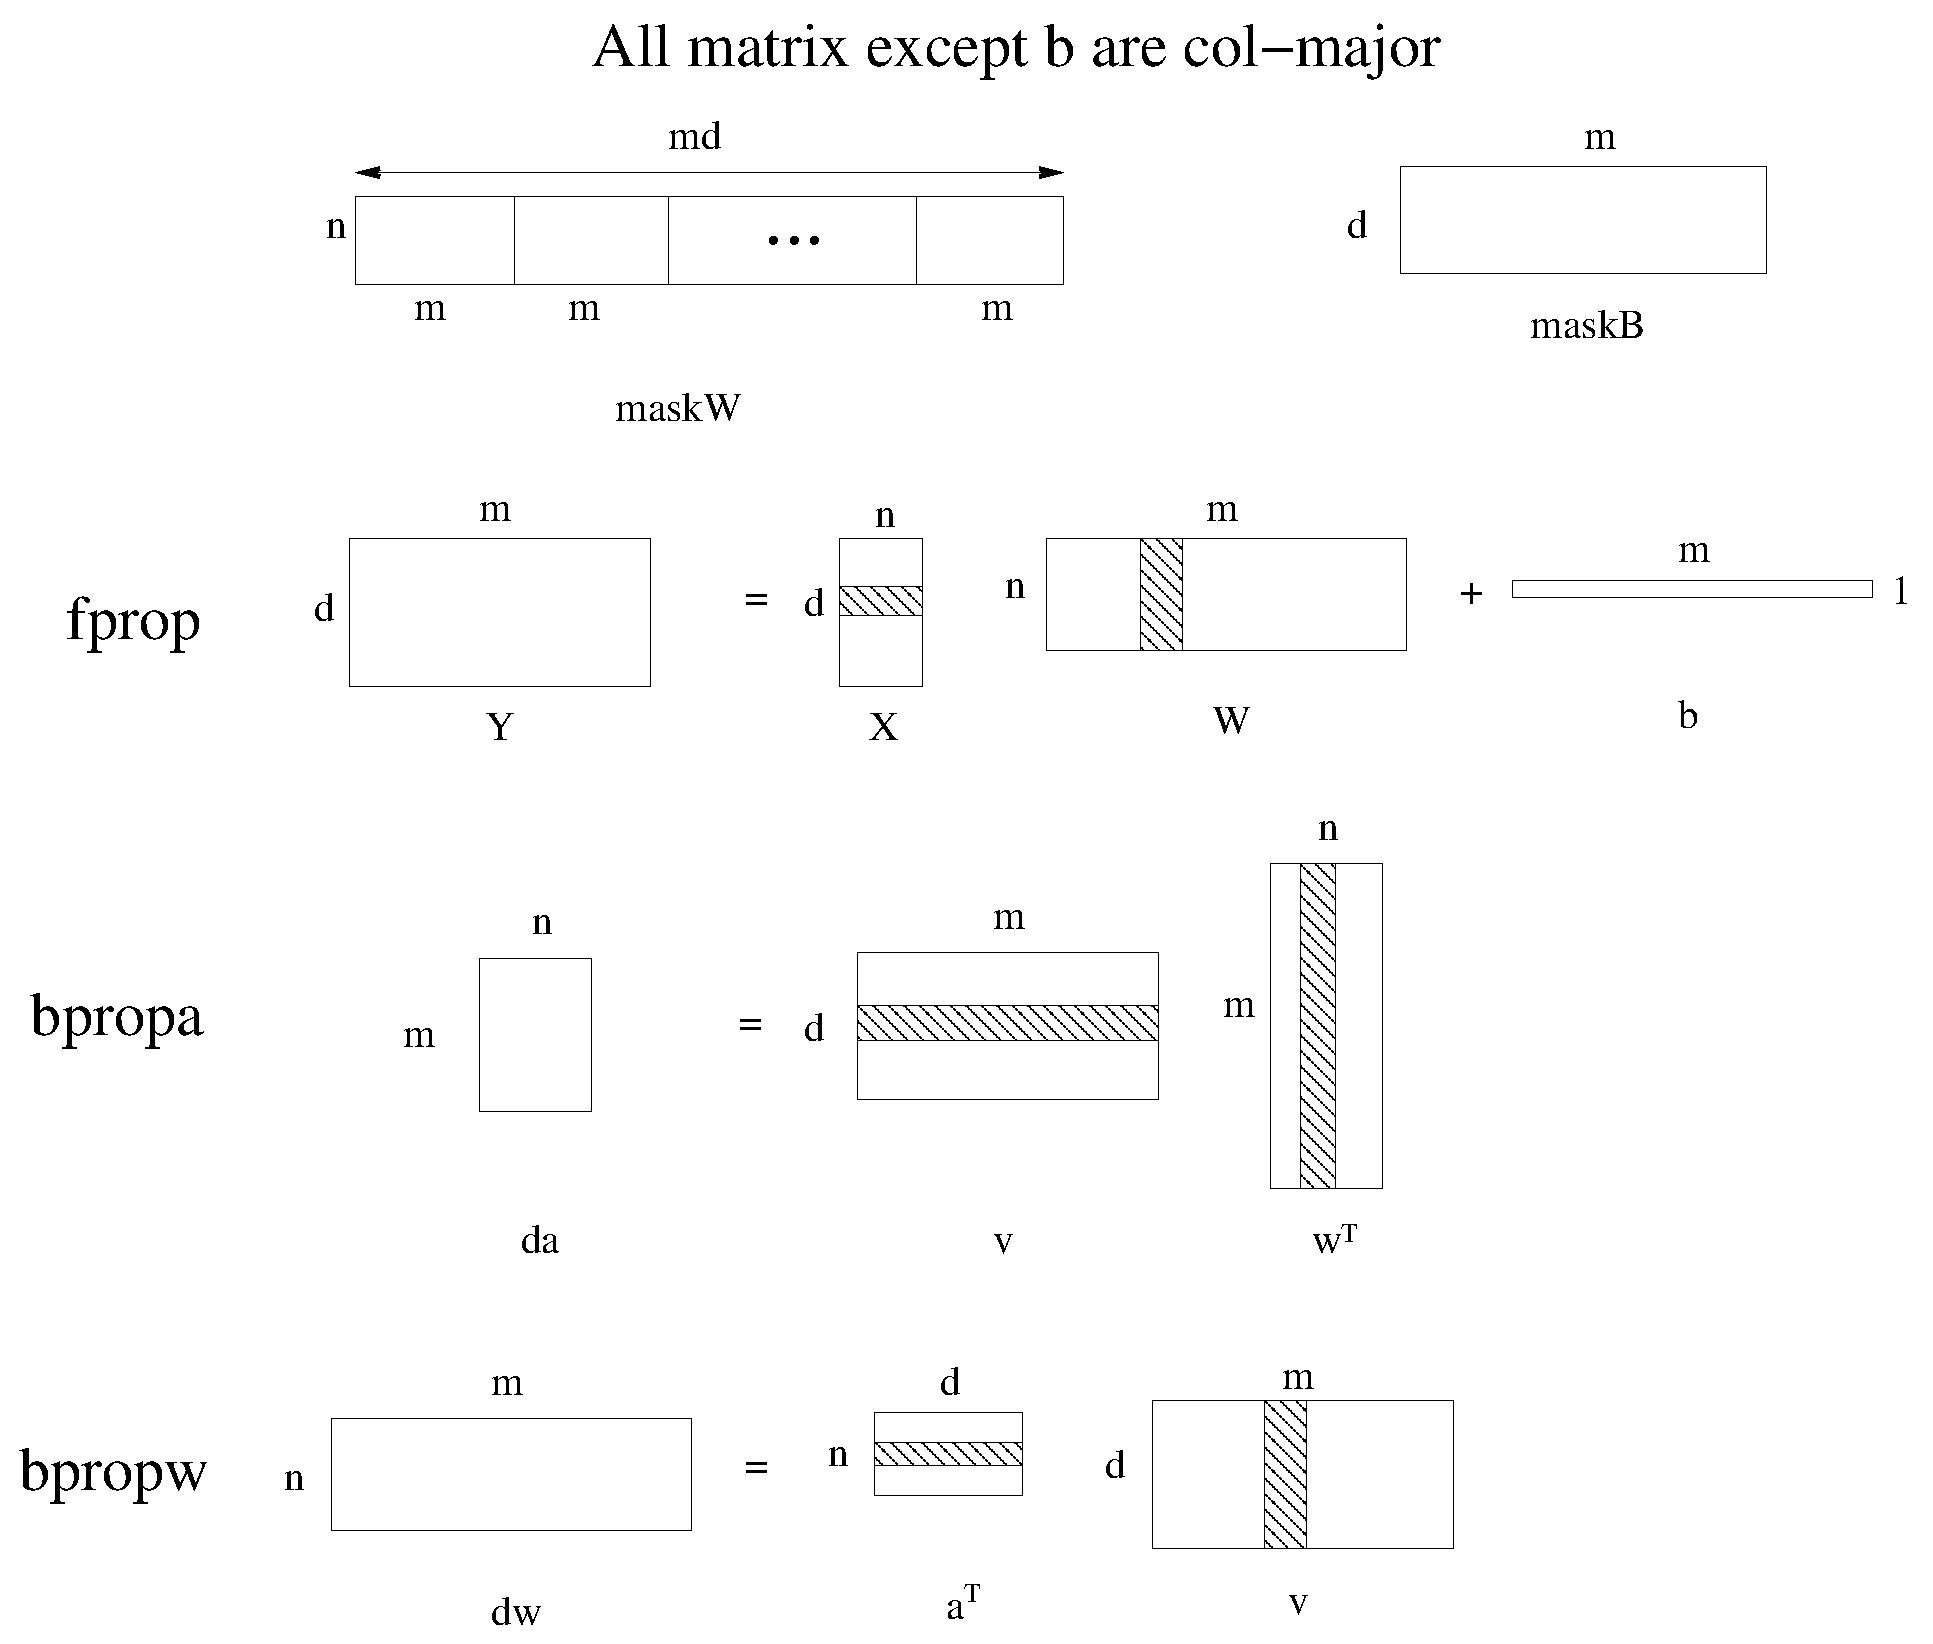
\includegraphics[width=4.5in]{figs/matrix_figure.eps}
%   }
%   \caption{
%      Device matrix memory memory layout
%   }
%\end{figure}
\begin{figure}[ht]
   \label{fig:gpu_memory_2}
   \centering{
      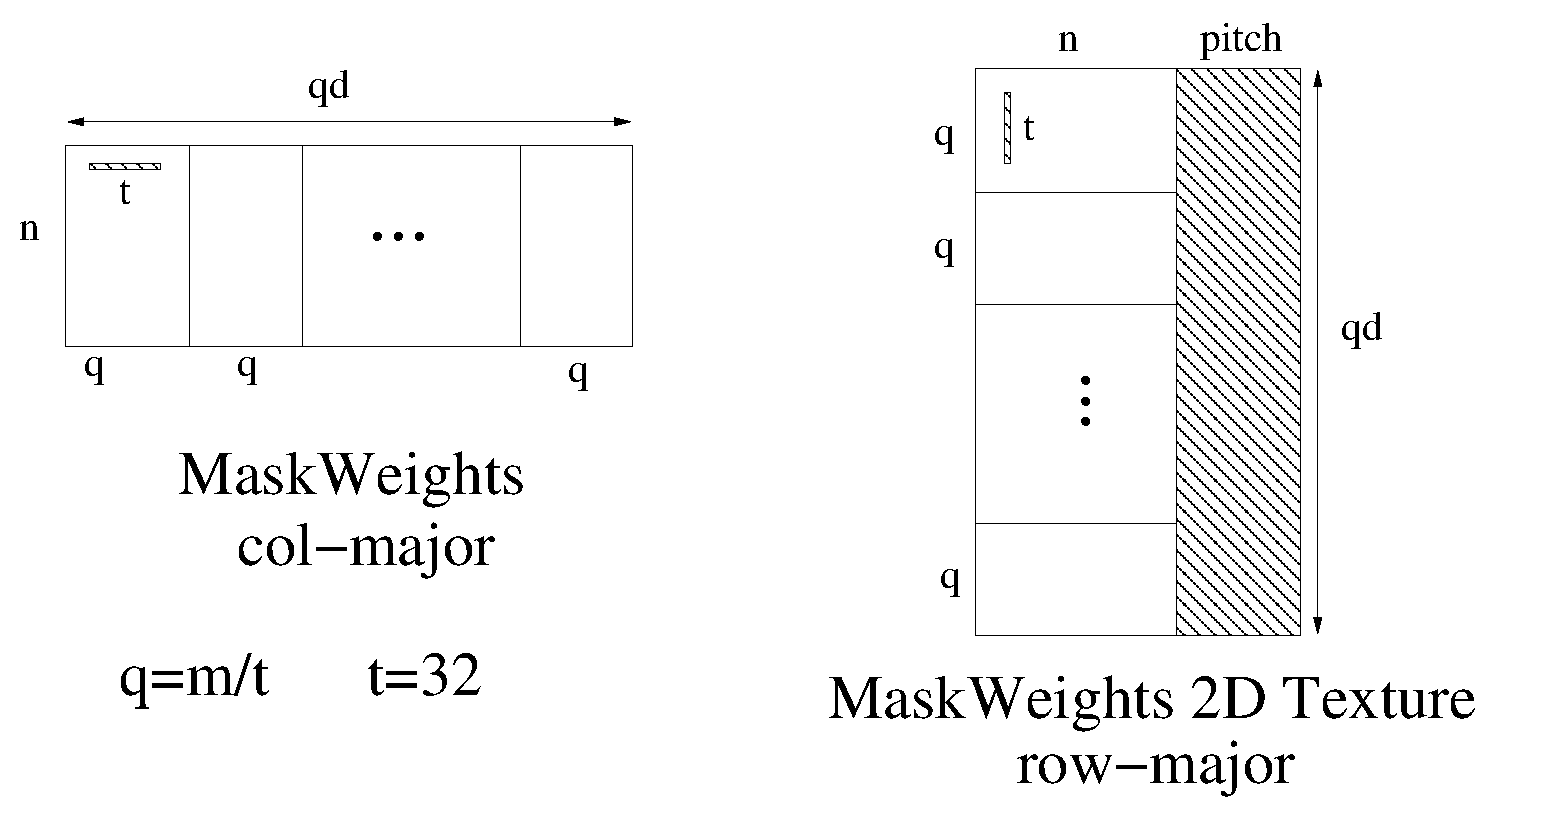
\includegraphics[width=4.5in]{figs/mw.eps}
   }
   \caption{
      Device mask weights memory layout
   }
\end{figure}
%----------------------------------------------
\section{Empirical Study}
\begin{table}[ht]
    \begin{center}
        \begin{tabular}{|l|l|l|l|l|l|l|l|p{3cm}|}
            \hline
            model & run-$1$ & run-$2$ & run-$3$ & run-$4$ & run-$5$ & mean/std & 5 model vote & voting performance boost \\
            \hline
            no drop & 11.15 & 11.11 & 11.33 & 11.03 & 11.30 & 11.18$\pm$ 0.13 & 10.22 & 0.96 \\
           drop out & 11.54 & 11.23 & 11.70 & 11.61 & 11.55 & 11.52$\pm$ 0.18 & 9.83 & 1.69 \\
    drop connect & 11.20 & 11.22 & 11.13 & 11.05 & 10.88 & 11.10$\pm$ 0.13 & {\bf 9.41} & 1.69 \\
            \hline
        \end{tabular}
    \end{center}
    \caption{
        Classification Performance on CIFAR-10 data set, previous state of the arts is $11.21\%$
        ~\cite{Schmidhuber2012}
    }
\end{table}
%----------------------------------------------
\bibliographystyle{plainnat}
\bibliography{refs}
\end{document}

